\documentclass[12pt,oneside,a4paper]{article}

\usepackage{./custom}

\newcommand{\question}[1]
{
\addtocounter{section}{1}
\paragraph*{Question \thesection}
\emph{\textcolor{red}{#1}}
}

\begin{document}
% title (fold)
\begin{center}
{\LARGE \bfseries 
 Questions et réponses exams de création d'entreprise \\[0.3cm] 
}
{\large
  \textsc{CentraleSupélec} --- Marc BATAILLOU ALMAGRO --- P2018\\[0.7cm]
}
\end{center}
% title (end)

%%%%%%%%%%%%%%%%%%%%%%%%%%%%%%%%%%%%%%%%%%%%%%%%%%%%%%%%%%%%%%%%%%%%%%%%%%%%%%%%%%%%
\question{Comment définir une entreprise solidaire et sociale ?}
On peut définir l'économie sociale et solidaire comme ``un mode d'entreprendre et de développement
économique adapté à tous les domaines de l'activité humaine, 
auquel adhèrent des personnes morales de droit privé qui remplissent les conditions cumulatives suivantes.''
Les entreprises solidaires et sociales partagent trois caractéristiques communes, à savoir
\begin{enumerate}
  \item un projet économiquement viable,
  \item une finalité associative,
  \item et une gouvernance participative (décisions prises collectivement, participation pas seulement en apport de capital).
\end{enumerate}
Dans ce type de projet, la finalité sociale dépasse la finalité économique.
On notera qu'il est donc plus difficile de convaincre les investisseurs.

%%%%%%%%%%%%%%%%%%%%%%%%%%%%%%%%%%%%%%%%%%%%%%%%%%%%%%%%%%%%%%%%%%%%%%%%%%%%%%%%%%%%
\question{En quoi le build-up est-il créateur de valeur ?}
Le \emph{build-up} est défini comme une ``suite d'acquisitions financées essentiellement
par endettement, menées par une entreprise reprise en LBO (Leveraged Buy Out) destinée 
à constituer un groupe plus important, plus rentable grâce aux synergies mises en oeuvre 
et donc avec une meilleure valorisation pour ses actionnaires lors de sa cession ultérieure.''
Cela permet une création de valeur par l'\emph{effet de taille}.
En effet, la PME de départ se retrouve structurée 
pour mieux \emph{résister à la concurrence} et entamer une nouvelle phase de croissance.
(On notera égalemment les avantages suivants : 
structuration des équipes et capacité à attirer de nouveaux talents,
capacités d’investissement et de développement accrues,
facilitation de l’accès à l’exportation, 
accès à de nouveaux clients/marchés jusque-là inaccessibles,
partage des meilleures pratiques entre les différentes entités du groupe,
synergies des coûts liés aux achats, accès plus facile aux crédits.)

%%%%%%%%%%%%%%%%%%%%%%%%%%%%%%%%%%%%%%%%%%%%%%%%%%%%%%%%%%%%%%%%%%%%%%%%%%%%%%%%%%%%
\question{Décrire un montage de type LBO.}
Le LBO (Leveraged Buy Out) désigne le rachat d'entreprise par effet de levier,
c'est-à-dire par recours à un fort endettement bancaire.
\begin{enumerate}
  \item Tout d'abord, les repreneurs vont créer une société (dite de \emph{holding})
  en faisant en sorte d'être majoritaire dans le capital.
  \item Ensuite, ce \emph{holding} fait en sorte d'être majoritaire dans la société
  convoitée et ce en utilisant le moins de fonds propres possible, mais surtout
  en utilisant l'argent d'un emprunt (appelé dette senior).
  \item Finalement, les charges financières des dettes contractées par la holding
  seront payées grâce aux \emph{remontées de dividendes} provenant de la cible. 
  Les repreneurs vont pouvoir acquérir la cible grâce aux ressources même de celle-ci.
\end{enumerate}
On retiendra deux avantages à ce montage
\begin{enumerate}
  \item L'emprunt de la holding est intégralement payé par le résultat de la cible.
  \item La holding pourra \emph{déduire de l’impôt} sur les sociétés les intérêts de 
  l’emprunt si elle détient une forte participation dans la société cible.
\end{enumerate}

%%%%%%%%%%%%%%%%%%%%%%%%%%%%%%%%%%%%%%%%%%%%%%%%%%%%%%%%%%%%%%%%%%%%%%%%%%%%%%%%%%%%
\question{Une entreprise qui décide de verser 10\% de ses bénéfices à des associations
humanitaires est-elle une entreprise solidaire et sociale ?}
\emph{Non}, ceci serait plus vu comme une \emph{action} solidaire et sociale,
sans pour autant changer le type d'entreprise.
On parle d'entreprise solidaire et sociale (voir définition plus haut)
lorsque 
\begin{enumerate}
  \item la \emph{finalité} est sociale avant d'être commerciale,
  \item la \emph{gouvernance} est de type participative,
  \item la \emph{lucrativité} est limitée (cette limite n'est pas clairement définie
  mais stipule que le but n'est pas de reverser les bénéfices aux actionnaires
  mais plutôt de les réinvestir dans son (ou bien des autres) activité sociale).
\end{enumerate}
 
%%%%%%%%%%%%%%%%%%%%%%%%%%%%%%%%%%%%%%%%%%%%%%%%%%%%%%%%%%%%%%%%%%%%%%%%%%%%%%%%%%%%
\question{Quels sont les différents stades de financement d’une entreprise, du point de vue du capital risque ? Quels types de risques un investisseur peut il être prêt à prendre ou au contraire à rejeter ?}


\vspace{1cm}
\begin{tabular}{|c|c|c|} 
	\hline
	 Phase & Montant sollicité & Cycle de vie\\
	 \hline
	 Pré-amorçage & <50K & < début activité comerciale\\
	 \hline
	 Capital amorçage & [50K,250K] & [début acti comerciale, 1.5ans ]\\
	 \hline
	 Capital création & [250K,500K] & [1.5 ans,seuil rentabilité ($\approx$4ans]\\
	 \hline
	 Capital développement & [500K, 1000K[ & >seuil rentabilité\\
	 \hline
\end{tabular} 
\vspace{1cm}

\fbox{
\begin{minipage}{\textwidth}
\noindent

\textbf{Pré-amorçage:} prêts familiaux; Prêts d'honneur \\
\textbf{Capital amorçage:} capital de proximité (love money, cigales..); Business Angels ; Incubateurs\\
\textbf{Capital création: }Business Angels ; Venture Corporate\\
\textbf{Capital développement:} Fonds de développement (Venture capital)\\

\end{minipage}
}

On peut aussi caractériser les entreprises avec d'autres indicateurs : 

\vspace{1cm}
\begin{center}
\begin{tabular}{|c|c|}
	\hline
	Stade & Risque\\
	\hline
	Concept défini : stade de l'idée & \\
	\hline
	Il existe un prototype : stade de produit & Risque produit\\
	\hline
	Produit industrialisé : stade industriel & Risque industriel\\
	\hline
	Premières ventes : première preuve de marché & Risque de marché\\
	\hline
	Nombreux clients ont acheté : repeat business & Risque d'éxecution\\
	\hline
	Expansion internationale: stade de déploiement international & \\
	\hline

\end{tabular}
\end{center}
\vspace{1cm}

\question{Peut on parler de relation client / fournisseur entre entrepreneurs et investisseurs en capital? Si oui, ou si non, pourquoi?}

\fbox{
\begin{minipage}{\textwidth}
\textbf{Non}. Les investisseurs \emph{apportent de l’argent à l’entreprise} (et non pas à l’entrepreneur) en participant à une \emph{augmentation de capital}. De ce fait, ils deviennent \textbf{actionnaires} de l’entreprise, au même titre que l’entrepreneur. Ils prennent par ailleurs une \emph{position capitalistique importante} (plusieurs dizaines de pourcents du capital, voire plus de 50$ \%$, au gré des refinancements). Ils négocient très souvent des droits particuliers au niveau de la gouvernance de l’entreprise et ont en quelque sorte un\emph{ `	statut' d’\textbf{associé}}. Ils participent, avec l’entrepreneur, au devenir de l’entreprise, pour \emph{le meilleur et pour le pire}.
\end{minipage}
}


\question{Qu’est-ce qu’une clause de buy or sell ? En quoi cette clause est elle importante pour un investisseur ?}

\fbox{
\begin{minipage}{\textwidth}
La clause de buy or sell est une clause \emph{quasi systématiquement présente} dans les pactes d’actionnaires. Elle assure aux investisseurs que les entrepreneurs financés feront leurs meilleurs efforts pour trouver une \textbf{liquidité} à leur investissement, dans un \emph{horizon de temps déterminé à l’avance}. Soit les \emph{entrepreneurs trouvent une liquidité} (sortie) pour les investisseurs, soit ces derniers sont \emph{autorisés à vendre la \textbf{totalité} (des actions)} de l’entreprise.
\end{minipage}
}

\question{A quoi et à qui peut servir un Business Model ? Quels sont les éléments nécessaires à sa construction ? }

\fbox{
\begin{minipage}{\textwidth}
Le Business Model modélise le fonctionnement de l’entreprise. Il doit donc comporter les éléments suivants :

\begin{itemize}[label=\ding{69}]
\item la manière dont l’entreprise \underline{produit de la valeur (schéma de production)}
\item la manière dont l’entreprise \underline{accède à ses clients (Go to market)}
\item la manière dont l’entreprise \underline{monétise son offre (Revenue model)}
\end{itemize}

en ayant précisé implicitement :

\begin{itemize}[label=\ding{69}]
\item qui sont les \textbf{clients de l’entreprise (segmentation)}
\item quel est le \textbf{positionnement de l’entreprise dans la chaîne de la valeur}
\end{itemize}

Le Business Model permet à l’entrepreneur \underline{formaliser} puis d’\underline{anticiper} le comportement économique de son entreprise, de \emph{tester des hypothèses}, de \emph{détecter les `sensibilités' ou zones de risque} de son entreprise.
Le Business Model permet aux \emph{investisseurs de mieux appréhender le fonctionnement} de l’entreprise.
\end{minipage}
}

\question{Sur quoi le créateur, et plus largement le dirigeant d’une entreprise, doit il garder l’œil rivé «en permanence»? (réponse en 1 mot)}

\fbox{
\begin{minipage}{\textwidth}
\textbf{La trésorerie.}
\end{minipage}
}


\question{Quel est le plan type d’un Business Plan ?}

\fbox{
\begin{minipage}{\textwidth}
Le \textbf{Business plan} décrit le projet de création d’entreprise. Il présente notamment :

\begin{itemize}[label=\ding{69}]
	\item L’historique du projet,
	\item Une analyse de marché,
	\item L’offre de l’entreprise et son positionnement par rapports aux offres concurrentes,
	\item Le Business Model de l’entreprise projetée,
	\item L’équipe en place et/ou à construire,
	\item Les chiffres clés passés et à venir,
	\item Le plan de financement.	
\end{itemize}

Le BP est structuré généralement en trois parties : Executive Summary (1 à 2 pages max), Corps du document (8-10 pages) Annexes.
\end{minipage}
}


\question{Quelles sont, selon Christophe Crémer, les quatre bases sur lesquelles toute action marketing doit s’appuyer ?}

\fbox{
\begin{minipage}{\textwidth}
\begin{itemize}[label=\ding{69}]
	\item Bénéfices clients
	\item Arguments d’autorité
	\item Incitation à passer à l’acte
	\item Nouveauté	
\end{itemize}
\end{minipage}
}

\question{Citez au moins quatre dispositifs publics ou associatifs d'aide à la création d'entreprises:}

\fbox{
\begin{minipage}{\textwidth}
\begin{itemize}[label=\ding{69}]
    \item PM'Up, par la Région Île-de-France
    \item Le PCE (Prêt à la Création d'Entreprise) de OSEO-Financement
    \item Le CDC (Contrat Développement Création) de OSEO-Financement
    \item Prêt d'honneur, du réseau Entreprendre
\end{itemize}
\end{minipage}
}

\question{Quels sont les différents segments (ou métiers) du private equity?}

\fbox{
\begin{minipage}{\textwidth}
\begin{itemize}[label=\ding{69}]
	\item Capital risque (amorçage et création)
    \item Capital-développement (renfort et d'expansion d'activité)
    \item Capital-transmission (entrées en bourse, leveraged buy-out, etc)
    \item Capital-retournement: entreprises en difficultés
\end{itemize}
\end{minipage}
}

\question{Selon Audrey Steward, qel est le prérequis le plus important avant de se lancer dans un projet d'entreprenariat?}

\fbox{
\begin{minipage}{\textwidth}
Faire un \underline{exit plan}, c'est à dire, prevoir la démarche à suivre si quelqu'un des créateurs décide de quitter l'entreprise.
\end{minipage}
}

\question{Faut-il toujours innover ?}

\fbox{
\begin{minipage}{\textwidth}
\textbf{Non.} Copier peut être une bonne idée (par exemple copier une entreprise aux USA).
\end{minipage}
}


\question{Selon Alain Crémer quel est l'élément clé de la réussite ?}

\fbox{
\begin{minipage}{\textwidth}
Le \textbf{marketing}, est la clé de la différenciation. De plus pour lui il faut toujours croire au succés, et alors on ne peut rater. 
\end{minipage}
}


\question{Que sont la chaine de valeur externe, et la chaine de valeur interne? (2 phrases ou exemple)}

\fbox{
\begin{minipage}{\textwidth}
\begin{itemize}[label=\ding{69}]
    \item Point de vue interne à l’entreprise : ensemble des activités (principales ou de soutien) qui concourent à la création de la valeur
    \item Point de vue externe à l’entreprise : ensemble des segments d’une filière qui concourent à la création de la  valeur
    \item Exemple : fabrication du pain
        \subitem +Achats des ingrédients, assemblage, pétrissage, cuisson, mise en magasin
        \subitem +Agriculteur, coopérative, meunier, transporteurs, boulangers
\end{itemize}
\end{minipage}
}


\question{Quels sont les clients d'un investisseur en capital? Quel est le service rendu par un investisseur à ses clients?}

\fbox{
\begin{minipage}{\textwidth}
Les services d'un investisseurs sont les souscripteurs au fond d'investissement. Il est important donc de comprendre que dans l'exemple des Venture Capital Funds, les clients ne sont pas les startups financées.
La prestation de l'investisseur est de gérer l'argent de ses clients, et de trouver des bonnes investissements avec un risque et un horizon de retour précédemment établis.
\end{minipage}
}
\vspace{1cm}

\textbf{\emph{Business model selon Alexander Osterwalder}}
\begin{figure}[h]
	\begin{center}
		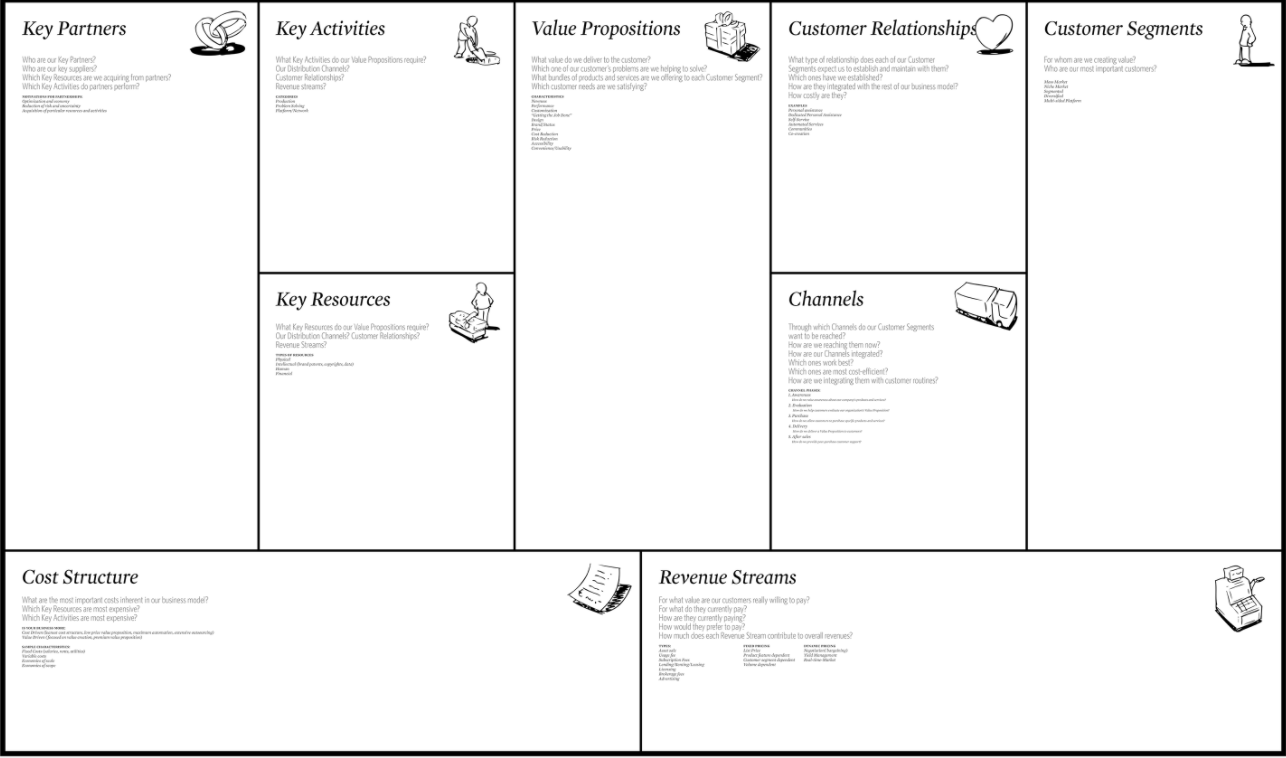
\includegraphics[scale=0.5]{./img/im1.png}
	\end{center}
\end{figure}



\end{document}